\newpage

\section{Results and discussion}
In this section the result of the simulations will be presented and discussed. Two different variations of the LB solver were tested. One with the optimised values of the relaxation parameters~\cite{geier:parameter} and other with the relaxation parameters used as specified in ~\cite{geier:cumulant}. The results presented in this section are performed with the former variation of the LB solver  and the results of the latter variation will just be presented in the Appendix, as the choice of value one for all the parameters is the most stable choice but not accurate enough~\cite{geier:parameter}. Firstly, the results of the LB simulations carried out without any turbulence model will be presented and discussed. The result of the simulations with no-model will be termed as the \emph{under resolved DNS} (UDNS). Under resolved because the resolution is coarser compared to the reference mesh resolution and DNS because no additional modelling is done for turbulence. It will be followed by the discussion of the results from the LB-LES with the WALE model and will be compared with the UDNS and DNS results. Few general comments applicable for all the simulations are:

\begin{itemize}
\item The DNS results of~\cite{kim:moin:moser:87} , for $Re_\tau = 395$, will be used as a reference for the comparison. The quantities obtained from the DNS data will be referred to as the \emph{target} quantities.
\item The results shown here are plotted against the global coordinates, $y/\de$, and local coordinates,  $y^+$.  
\item All simulations have been performed using the single precision on GPGPUs
\item The normalised wall distance $y^+$ used in the profile plots is computed aposteriori for all the simulations.
\end{itemize}

\subsection{UDNS results}
The physical quantities resulting from the simulations viz. $u_\tau$, $Re_\tau$ for all meshes will be compared with the corresponding target values from the DNS data. Mesh 1 predicts the lowest value of the $u_\tau$ in comparison to other mesh resolutions, when compared with the target value of $u_\tau$.  The following table (\ref{Global quantities}) shows the comparison with the target values:
%
\begin{table}[h!]
\begin{center}
\begin{tabular}{ p{3cm}|p{1.5cm}p{1.5cm}p{1.5cm}p{1.5cm}  } 
\hline
Physical quantity & Mesh1 & Mesh1\_5 & Mesh2 & Target \\
  \hline
  \multirow{1}{6em}{$u_\tau,\ m/s$}  & 0.0070 & 0.0074 & 0.0076 & 0.0079\\
  \hline
  \multirow{1}{6em}{$Re_\tau$} & 352 & 371 & 382 & 395\\
  \hline
  \multirow{1}{6em}{$U_c,\ m/s$} & 0.1565 & 0.1563 & 0.1557 & 0.1591\\
  \hline
\end{tabular}
\end{center}
\caption{Comparison of the resulting physical quantities}
\label{Global quantities}
\end{table}\\
%
\begin{figure}[t]
    \centering
    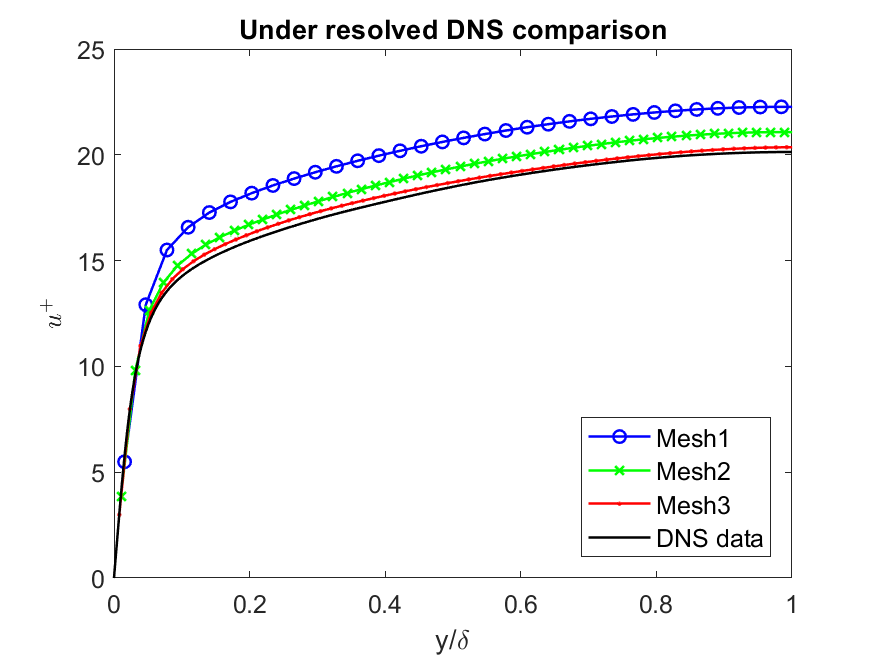
\includegraphics[width=1\textwidth]{06_Resultsanddiscussion/figur/UDNS_2016/Profile_global_coords.png}
    \caption{Mean velocity profile normalized by $u_\tau$ in global coordinates}
    \label{Mean velocity global}
\end{figure}

\begin{figure}[h]
    \centering
    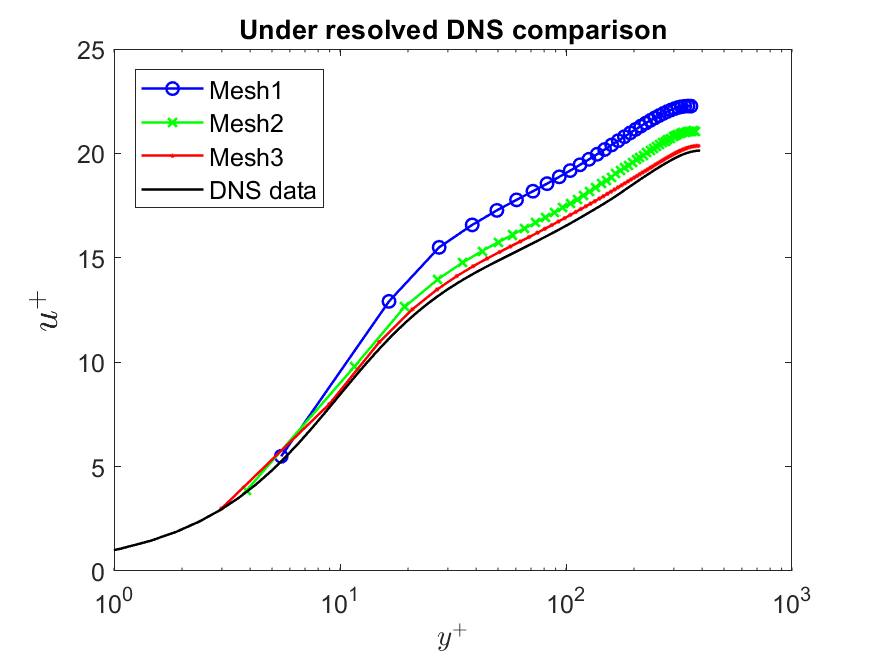
\includegraphics[width=1\textwidth]{06_Resultsanddiscussion/figur/UDNS_2016/Profile_wall_coords_theo_comp.png}
    \caption{Mean velocity profile normalized by $u_\tau$ in wall coordinates}
    \label{Mean velocity wall}
\end{figure}

As stated before the simulations have been performed on three different mesh resolutions. The results of the UDNS are presented in the form of mean velocity and the Reynolds stress profiles. In these plots, the comparison of the different mesh resolution with each other as well as with the DNS data is shown. Figure (\ref{Mean velocity global}) shows the mean velocity profiles in global coordinates. It can be seen from the comparison of the profiles that with the increase in the mesh resolution the profile approaches closer to the DNS profile. 
Fiction velocity $u_\tau$ is the averaged value.From table (\ref{Global quantities}) we can see that the averaged $u_\tau$ increases with the mesh resolution and tend towards the target $u_\tau$ and so is for the $Re_\tau$.   friction velocity 